%-----------------------------------------------------------------------------------------------
\documentclass[12pt,aspectratio=169]{beamer}
%-----------------------------------------------------------------------------------------------
\usepackage{pslatex}
\usepackage[greek,french,english,brazil]{babel} % last becomes the active one
\usepackage{ulem}
\renewcommand{\ULdepth}{3.0pt}
%-----------------------------------------------------------------------------------------------
\newcommand{\YA}{%
    \mbox{%
        Y\makebox[0pt][l]{\hspace{-0.178em}\raisebox{-0.00ex}{\scalebox{0.30}{E}}}%
        H\makebox[0pt][l]{\hspace{-0.010em}\raisebox{-0.00ex}{\scalebox{0.30}{O}}}%
        W\makebox[0pt][l]{\hspace{-0.245em}\raisebox{-0.00ex}{\scalebox{0.30}{A}}}%
        H%
    }%
}
%-----------------------------------------------------------------------------------------------
\newcommand{\ver}[1]{%
    \raisebox{0.50ex}{%
        \scalebox{1.1}{%
            \pmb{\textbf{\textcolor{BSpbg}{#1}}}%
        }%
    }%
}
%-----------------------------------------------------------------------------------------------
\newcommand{\QUOTE}[1]{%
    \par\noindent\hspace*{0.1\linewidth}%
    \begin{minipage}{0.8\linewidth}%
        \linespread{1.35}\large{#1}%
    \end{minipage}%
}
%-----------------------------------------------------------------------------------------------
\newcommand{\WIDEQUOTE}[1]{%
    \par\noindent\hspace*{0.02\linewidth}%
    \begin{minipage}{0.92\linewidth}%
        \linespread{1.25}\large{#1}%
    \end{minipage}%
}
%-----------------------------------------------------------------------------------------------
\newcommand{\RED}[1]{{\textcolor{TXred}{#1}}}
\newcommand{\ORA}[1]{{\textcolor{TXora}{#1}}}
\newcommand{\YEL}[1]{{\textcolor{TXyel}{#1}}}
\newcommand{\GRE}[1]{{\textcolor{TXgre}{#1}}}
\newcommand{\CYA}[1]{{\textcolor{TXcya}{#1}}}
\newcommand{\BLU}[1]{{\textcolor{TXblu}{#1}}}
\newcommand{\MAG}[1]{{\textcolor{TXmag}{#1}}}
\newcommand{\BRI}[1]{{\textcolor{BSpbg}{#1}}}   % Bright
%-----------------------------------------------------------------------------------------------
\newcommand{\ENtxt}[1]{\begin{otherlanguage}{english}{{#1}}\end{otherlanguage}}
\newcommand{\GRtxt}[1]{\begin{otherlanguage}{greek}{{#1}}\end{otherlanguage}}
\newcommand{\FRtxt}[1]{\begin{otherlanguage}{french}{{#1}}\end{otherlanguage}}
%-----------------------------------------------------------------------------------------------
\usetheme{CambridgeUS}
\usefonttheme{serif}
\usecolortheme{BShare1}
%-----------------------------------------------------------------------------------------------
\title{Estudo do \textit{Timing} em Mt 24.1--14}
\subtitle{Parte A --- O ``Fim'' em Mateus~24}
\author{Bíblia Share}
%\institute{Bíblia Share}
\date[{\tiny\tt{26 de fevereiro de 2022}}]{{\scriptsize\tt%
    \includegraphics[height=6.0mm]{res/cc/by-nc-88x31.pdf}\\[\smallskipamount]
    26 de fevereiro de 2022%\today
}}
%-----------------------------------------------------------------------------------------------
\begin{document}
%-----------------------------------------------------------------------------------------------
\logo{%
    \parbox{158mm}{% There's a 1mm gap on each side of the 160mm x 90mm slide logo line
    \mode<beamer>{%
        \hfill\includegraphics[height=9.0mm]{res/logo/BibliaShare.pdf}%
    }
    \mode<handout>{%
        \hfill\includegraphics[height=9.0mm]{res/logo/BibliaShare.pdf}%
    }
}}
%-----------------------------------------------------------------------------------------------
\begin{frame}
    \titlepage
\end{frame}
%%%-----------------------------------------------------------------------------------------------
%%\section{Verso Base}
%%%-----------------------------------------------------------------------------------------------

    \begin{frame}
        \QUOTE{%
            %-----!j 92 -i12
            \ver{(ARA) Mt~24.2}~%
            Ele, porém, lhes disse: \YEL{Não vedes tudo  isto?}  Em  verdade  vos  digo  que
            \YEL{não ficará aqui pedra sobre pedra que não seja derribada.}
        }
    \end{frame}

    \begin{frame}
        \QUOTE{%
            %-----!j 92 -i12
            \ver{(ARA) Mt~24.3}~%
            No monte das Oliveiras, achava-se Jesus assentado, quando se aproximaram dele os
            discípulos, \BRI{em particular}, e lhe pediram: Dize-nos  \YEL{quando  sucederão
            estas coisas} e \GRE{que sinal haverá da tua  vinda}  e  da  \MAG{consumação  do
            século}.
        }
    \end{frame}

    \begin{frame}
        \QUOTE{%
            %-----!j 92 -i12
            \ver{(ARA) Dn~9.20a}~%
            Falava eu ainda, e orava, e confessava o meu pecado e o pecado do \YEL{meu  povo
            de Israel} [...] \\[\bigskipamount]
            %-----!j 92 -i12
            \ver{(ARA) Dn~9.24}~%
            \GRE{Setenta semanas} estão \MAG{determinadas} sobre \YEL{o teu  povo}  e  sobre
            \ORA{a tua santa cidade}, para fazer cessar a transgressão,  para  dar  fim  aos
            pecados, para \BRI{expiar a iniquidade}, para  \BRI{trazer  a  justiça  eterna},
            para selar a visão e a profecia e para ungir o Santo dos Santos.
        }
    \end{frame}

    \begin{frame}
        \QUOTE{%
            %-----!j 92 -i12
            \ver{(ARA) Mt~24.15}~%
            \YEL{Quando}, pois, virdes \GRE{o  abominável  da  desolação}  de  que  falou  o
            \MAG{profeta Daniel}, no lugar santo (quem lê entenda),
        }
    \end{frame}

    \begin{frame}
        \QUOTE{%
            %-----!j 92 -i12
            \ver{(ARA) At~17.11}~%
            Ora, estes de \YEL{Bereia} eram \GRE{mais nobres} que os  de  Tessalônica;  pois
            receberam a palavra com toda a avidez, \MAG{examinando as  Escrituras  todos  os
            dias para ver se as coisas eram, de fato, assim}.
        }
    \end{frame}

    \begin{frame}
        \QUOTE{%
            %-----!j 92 -i12
            \ver{(ARA) Mt~24.15}~%
            \YEL{Quando}, pois, virdes \GRE{o  abominável  da  desolação}  de  que  falou  o
            \MAG{profeta Daniel}, no lugar santo (quem lê entenda), [...] \\[\bigskipamount]
            %-----!j 92 -i12
            \ver{(ARA) Mt~24.21}~%
            porque \YEL{nesse tempo} haverá \RED{grande tribulação}, como desde o  princípio
            do mundo até agora não tem havido e nem haverá jamais.
        }
    \end{frame}

    \begin{frame}
        \QUOTE{%
            %-----!j 92 -i12
            \ver{(ARA) Mt~24.15}~%
            \YEL{Quando}, pois, virdes \GRE{o  abominável  da  desolação}  de  que  falou  o
            \MAG{profeta Daniel}, no lugar santo (quem lê entenda), \\[\bigskipamount]
            %-----!j 92 -i12
            \ver{(ARA) Dn~9.27}~%
            Ele fará firme aliança com muitos, por uma semana; \YEL{na  metade  da  semana},
            fará cessar  o  sacrifício  e  a  oferta  de  manjares;  sobre  a  \GRE{asa  das
            abominações virá o assolador}, até que a destruição, que  está  determinada,  se
            derrame sobre ele.
        }
    \end{frame}

    \begin{frame}
        \QUOTE{%
            %-----!j 92 -i12
            \ver{(ARA) Mt~24.21}~%
            porque \YEL{nesse tempo} haverá \RED{grande tribulação}, como desde o  princípio
            do mundo até agora não tem havido e nem haverá jamais. \\[\bigskipamount]
            %-----!j 92 -i12
            \ver{(ARA) Dn~9.27}~%
            Ele fará firme aliança com muitos, por uma semana; \YEL{na  metade  da  semana},
            fará cessar  o  sacrifício  e  a  oferta  de  manjares;  sobre  a  \GRE{asa  das
            abominações virá o assolador}, até que a destruição, que  está  determinada,  se
            derrame sobre ele.
        }
    \end{frame}

    \begin{frame}
        \QUOTE{%
            %-----!j 92 -i12
            \ver{(A21) Mt~24.3}~%
            [...] seus discípulos  aproximaram-se  dele  em  particular,  dizendo:  Dize-nos
            \YEL{quando essas coisas acontecerão} e \GRE{que sinal haverá da tua vinda} e do
            \MAG{fim do mundo}. \\[\bigskipamount]
            %-----!j 92 -i12
            \ver{(ARC) Mt~24.3}~%
            [...] chegaram-se a ele os seus discípulos,  em  particular,  dizendo:  Dize-nos
            \YEL{quando serão essas coisas} e \GRE{que sinal  haverá  da  tua  vinda}  e  do
            \MAG{fim do mundo}?
        }
    \end{frame}

    \begin{frame}
        \QUOTE{%
            %-----!j 92 -i12
            \ver{(ARA) Ap~20.11}~%
            Vi um \BRI{grande trono branco} e \BRI{aquele que  nele  se  assenta},  de  cuja
            presença \YEL{fugiram} a \GRE{terra} e o \CYA{céu}, e \MAG{não  se  achou  lugar
            para eles}.
        }
    \end{frame}

    \begin{frame}
        \QUOTE{%
            %-----!j 92 -i12
            \ver{(ARA) Mt~24.3}~%
            No monte das Oliveiras, achava-se Jesus assentado, quando se aproximaram dele os
            discípulos, \BRI{em particular}, e lhe pediram: Dize-nos  \YEL{quando  sucederão
            estas coisas} e \GRE{que sinal haverá da tua  vinda}  e  da  \MAG{consumação  do
            século}.
        }
    \end{frame}

    \begin{frame}
        \QUOTE{%
            %-----!j 92 -i12
            \ver{(SBL) Mt~24.3}~%
            \GRtxt{Καθημένου δὲ αὐτοῦ ἐπὶ τοῦ Ὄρους τῶν Ἐλαιῶν  προσῆλθον  αὐτῷ  οἱ  μαθηταὶ
            κατ’ ἰδίαν λέγοντες· Εἰπὸν ἡμῖν \YEL{πότε ταῦτα ἔσται}, καὶ \GRE{τί  τὸ  σημεῖον
            τῆς σῆς παρουσίας} καὶ \MAG{συντελείας τοῦ αἰῶνος}}.
            % THANKS to https://jwodder.github.io/kbits/posts/unicode-latex/
        }
    \end{frame}

    \begin{frame}
        \begin{center}
            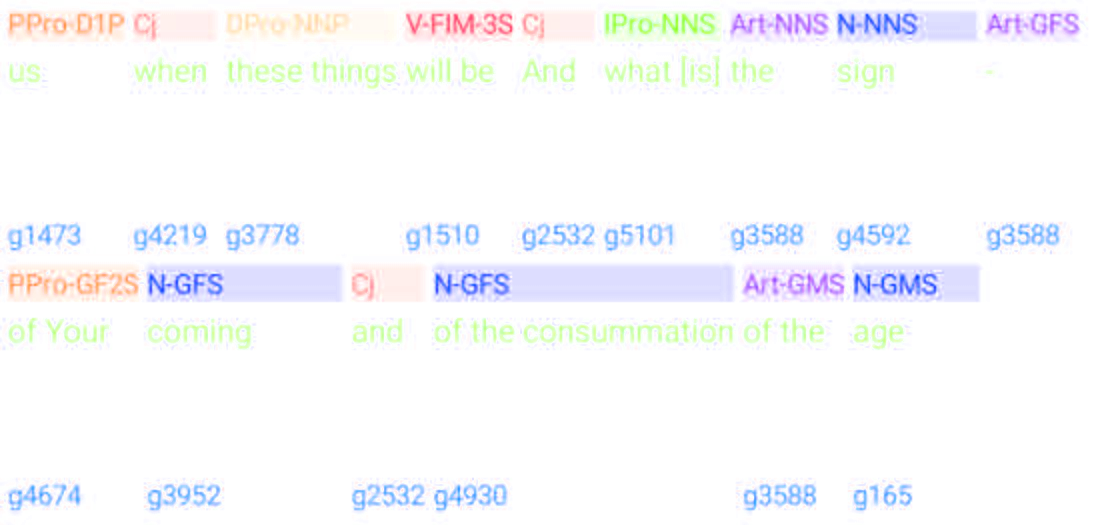
\includegraphics[width=128mm]{fig/Mt24-Greek-Crop-Alpha.png}
        \end{center}
    \end{frame}

    \begin{frame}
        \QUOTE{%
            %-----!j 92 -i12
            \ver{(ARA) Mt~25.46}~%
            E irão estes para o \RED{castigo eterno}, porém  os  justos,  para  a  \GRE{vida
            eterna}.
        }
    \end{frame}

    \begin{frame}
        \WIDEQUOTE{%
            %-----!j 92 -i12
            \ver{(ARA) Ap~19.19,20}~%
            E vi a \YEL{besta} e os reis da terra,  com  os  seus  exércitos,  [...]  contra
            \BRI{aquele que estava montado no  cavalo}  e  contra  o  seu  exército.  Mas  a
            \YEL{besta} foi aprisionada, e com ela o \ORA{falso profeta} que  [...]  seduziu
            aqueles que receberam a \MAG{marca da besta} e eram os  adoradores  da  \GRE{sua
            imagem}. \\[\bigskipamount]
            %-----!j 92 -i12
            \ver{(ARA) Ap~20.4}~%
            Vi ainda [...] tantos  quantos  não  adoraram  a  \YEL{besta},  nem  tampouco  a
            \GRE{sua imagem},  e  não  receberam  a  \MAG{marca  na  fronte  e  na  mão};  e
            \BRI{viveram e reinaram com Cristo durante mil anos}.
        }
    \end{frame}

    \begin{frame}
        \WIDEQUOTE{%
            %-----!j 92 -i12
            \ver{(ARA) Ap~19.19,20}~%
            E vi a \YEL{besta} e os reis da terra,  com  os  seus  exércitos,  [...]  contra
            \BRI{aquele  que  estava  montado  no  cavalo}  [...]  Mas  a  \YEL{besta}   foi
            aprisionada, e com ela o \ORA{falso profeta}  [...]  Os  \YEL{do}\ORA{is}  foram
            lançados vivos dentro do lago de fogo [...]
            \\[\bigskipamount]
            %-----!j 92 -i12
            \ver{(ARA) Ap~20.2,4}~%
            Ele prendeu o \RED{dragão}, a \RED{antiga  serpente},  que  é  o  \RED{diabo}  e
            \RED{Satanás}, e amarrou-o por mil anos. [...] Vi ainda [...] tantos quantos não
            adoraram a \YEL{besta}, nem tampouco a  \GRE{sua  imagem},  e  não  receberam  a
            \MAG{marca na fronte e na mão}; e \BRI{viveram e reinaram com Cristo durante mil
            anos}.
        }
    \end{frame}

    \begin{frame}
        \QUOTE{%
            %-----!j 92 -i12
            \ver{(ARA) Ap~20.4}~%
            Vi também tronos, e nestes sentaram-se aqueles aos quais foi dada autoridade  de
            julgar. Vi ainda as almas dos decapitados por causa do testemunho de Jesus,  bem
            como por causa da palavra de Deus, tantos quantos  não  adoraram  a  besta,  nem
            tampouco a sua  imagem,  e  não  receberam  a  marca  na  fronte  e  na  mão;  e
            \BRI{viveram e reinaram com Cristo durante mil anos}.
        }
    \end{frame}

    \begin{frame}
        \QUOTE{%
            %-----!j 92 -i12
            \ver{(ARA) 2Ts~2.7,8}~%
            Com efeito, o mistério da  iniquidade  já  opera  e  \YEL{aguarda  somente}  que
            \GRE{seja afastado} aquele que \GRE{agora o detém}; \MAG{então, será,  de  fato,
            revelado} o \RED{iníquo}, a quem o Senhor Jesus matará com o sopro de sua boca e
            o destruirá pela manifestação de sua vinda.
        }
    \end{frame}

%%%-----------------------------------------------------------------------------------------------
%%\section{Referências}
%%%-----------------------------------------------------------------------------------------------

%%    %------------------------------------------------------------------------------------------
%%    \begin{frame}[allowframebreaks]{Referências -- }
%%        \bibliographystyle{unsrt}
%%        \setbeamertemplate{bibliography item}{\insertbiblabel}
%%        \bibliography{bibfile.bib}
%%    \end{frame}
%%    %------------------------------------------------------------------------------------------

%-----------------------------------------------------------------------------------------------
\end{document}
%-----------------------------------------------------------------------------------------------
